%%%%%%%%%%%%%%%%%%%%%%%%%%%%%%%%%%%%%%%%%%%%%%%%%%%%%%%%%%%%%%%%%%%%%%%%%%%%%%%%%%%%%%%%%%%%%%%%%%%%%%%%%%%%%%%%%%%%%%%%%%%%%%%%%%%%%%%%%%%%%%%%%%%%%%%%%%%%%%%%%%%%%%%%%%%%%%

\UC{Checkout}

\begin{figure}[H]
    \centering
    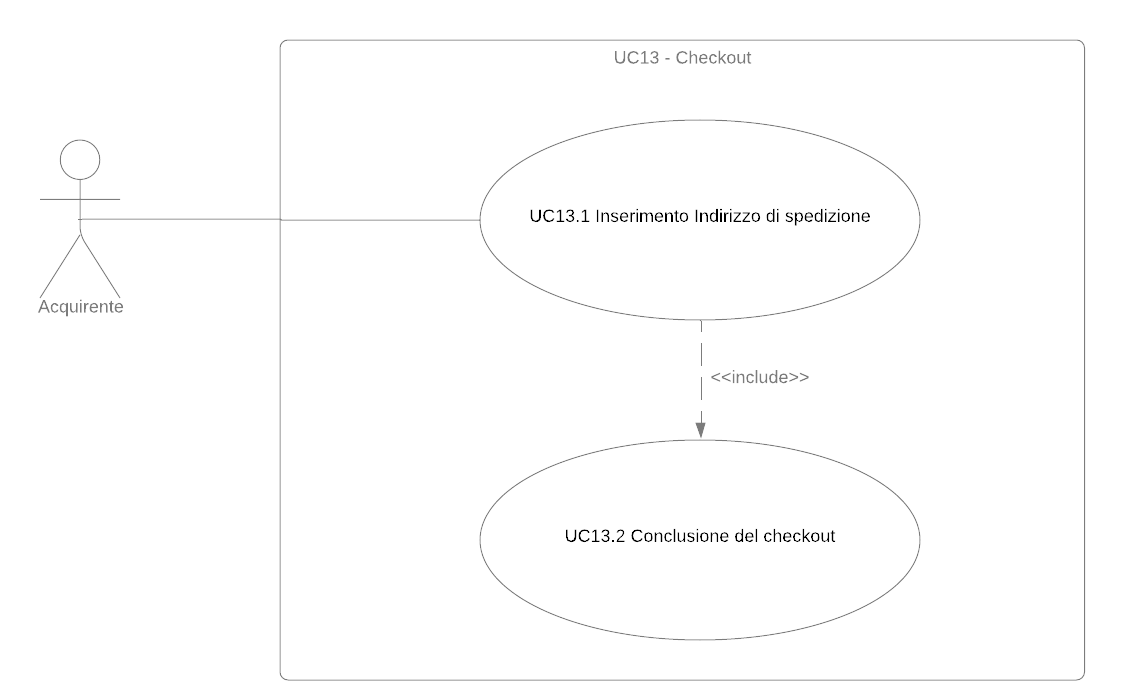
\includegraphics[scale=0.4]{Immagini/DiagrammiUC/UC13Checkout.png}
    \caption{Diagramma di \actualUC: Checkout} 
    \label{fig:Checkout}
\end{figure}

L'utente si trova nella schermata del carrello e vuole procedere al checkout per acquistare i prodotti scelti.
\begin{itemize}
    \item \textbf{Attori primari:} acquirente;
    \item \textbf{Attori secondari:} stripe;
    \item \textbf{Precondizione:} l'attore si trova nella schermata del carrello;
    \item \textbf{Postcondizione:} l'attore ha terminato il checkout e visualizza il riepilogo ordine.
    \item \textbf{Scenario principale:} l'attore si trova nella schermata del carrello e seleziona la funzionalità per procedere con il checkout. In seguito eseguirà le seguenti azioni:
    \begin{itemize}
    	\item (\actualUC.1) - selezionare l'indirizzo di consegna;
    	\item (\actualUC.2) - selezionare la carta con la quale svolgere il pagamento tra quelle inserite precedentemente;
    	\item inserire possibili informazioni aggiuntive per la consegna dell'acquisto;
        \item (\actualUC.3) - inviare il pagamento.
    \end{itemize} 
    \item \textbf{Scenari alternativi}: 
    \begin{enumerate}[label=\lett]
        \item l'attore vuole svolgere l'operazione di checkout ma non è ancora autenticato. Per questo motivo verrà reindirizzato alla schermata di login per potersi autenticare come acquirente, per poi procedere in seguito al checkout. Se l'utente accede come venditore, il carrello con i prodotti salvati verrà svuotato e andrà perso;
        \item se non è presente alcuna carta per il pagamento, allora verrà mostrato un messaggio il quale indicherà l'obbligo di dover inserire una carta per il pagamento per poter proseguire con il checkout. In seguito quella carta verrà selezionata automaticamente per proseguire con il pagamento;
        \item se non è presente alcuna carta da utilizzare per il pagamento, allora verrà mostrato un messaggio il quale indicherà l'obbligo di dover inserire un indirizzo di consegna per poter proseguire con il checkout. In seguito dell'indirizzo verrà selezionato automaticamente per proseguire con la consegna;
    \end{enumerate}
\end{itemize}

\resetSubUC

\subUC{Selezione dell'indirizzo della consegna}
L'acquirente seleziona l'indirizzo della consegna, ovvero dove verrà recapitato l'acquisto, tra gli indirizzi di consegna precedentemente inseriti.
\begin{itemize}
    \item \textbf{Attori primari:} acquirente e Stripe;
    \item \textbf{Precondizione:} l'acquirente non ha ancora pagato e il carrello non è vuoto;
    \item \textbf{Postcondizione:} l'acquirente ha effettuato il pagamento, il suo carrello è vuoto e si trova sulla pagina di riepilogo dell'ordine;
    \item \textbf{Scenario principale:}
        \begin{itemize}
            \item l'acquirente viene indirizzato alla pagina di checkout di Stripe, dove pagherà il costo del carrello più le spese di spedizione e le tasse;
            \item Stripe si occupa del pagamento;
            \item Quando è avvenuto il pagamento viene svuotato il carrello e gli articoli che lo componevano vengono sottratti nella quantità acquistata da quelli disponibili;
            \item Viene visualizzato il riepilogo ordine.
        \end{itemize}
    \item \textbf{Scenario alternativo:} Se il pagamento fallisce l'utente viene riportato alla pagina del carrello, senza che questo venga svuotato.
\end{itemize}

\subUC{Invio del pagamento}
L'acquirente procede al pagamento attraverso il servizio fornito da Stripe e poi gli viene mostrata una pagina con il resoconto dell'ordine.
\begin{itemize}
    \item \textbf{Attori primari:} acquirente e Stripe;
    \item \textbf{Precondizione:} l'acquirente non ha ancora pagato e il carrello non è vuoto;
    \item \textbf{Postcondizione:} l'acquirente ha effettuato il pagamento, il suo carrello è vuoto e si trova sulla pagina di riepilogo dell'ordine;
    \item \textbf{Scenario principale:}
        \begin{itemize}
            \item l'acquirente viene indirizzato alla pagina di checkout di Stripe, dove pagherà il costo del carrello più le spese di spedizione e le tasse;
            \item Stripe si occupa del pagamento;
            \item Quando è avvenuto il pagamento viene svuotato il carrello e gli articoli che lo componevano vengono sottratti nella quantità acquistata da quelli disponibili;
            \item Viene visualizzato il riepilogo ordine.
        \end{itemize}
    \item \textbf{Scenario alternativo:} Se il pagamento fallisce l'utente viene riportato alla pagina del carrello, senza che questo venga svuotato.
\end{itemize}

%%%%%%%%%%%%%%%%%%%%%%%%%%%%%%%%%%%%%%%%%%%%%%%%%%%%%%%%%%%%%%%%%%%%%%%%%%%%%%%%%%%%%%%%%%%%%%%%%%%%%%%%%%%%%%%%%%%%%%%%%%%%%%%%%%%%%%%%%%%%%%%%%%%%%%%%%%%%%%%%%%%%%%%%%%%%%%
